%%%%%Präambel%%%%%

\documentclass[12pt,a4paper]{article}%Schriftgröße, Papierformat einstellen
%\documentclass{scrbook}
\usepackage[top=30mm,bottom=30mm]{geometry}
\usepackage{lipsum}
\usepackage{csquotes}
%Pakete laden zur deutschen Rechtschreibung und für Umlaute
\usepackage[T1]{fontenc}
\usepackage[ngerman]{babel}
\usepackage[utf8]{inputenc} %für Windows, Linux
%\usepackage[applemac]{inputenc} %für Mac
%\usepackage{xcolor}
\usepackage[official]{eurosym}
\usepackage{graphicx}
\usepackage{caption}
\usepackage[dvipsnames]{xcolor}
\usepackage{cancel}
\usepackage{titlesec}
\usepackage{cite}
\usepackage{filecontents}
\usepackage{tabularx}
\usepackage{harvard}
\usepackage{units}
\usepackage{longtable} 
\usepackage{multirow}
\usepackage{chngcntr}
\usepackage{stmaryrd}
\usepackage{array}
\usepackage{autobreak}
\usepackage{booktabs}
\usepackage{float}
\usepackage{wrapfig}
\usepackage{hhline}
\let\harvardleftorig\harvardleft
%\usepackage[round]{natbib}
%\usepackage{hyperref}
\usepackage[nottoc,numbib]{tocbibind}
\usepackage{siunitx}
\usepackage{esvect}

%Pakete laden zu mathematischen Symbolen etc.
\usepackage{calc} 
\usepackage{amsmath,amssymb,amsthm}
\usepackage{scrpage2}
\pagestyle{scrheadings}
\clearscrheadfoot
\automark[chapter]{section}
\ofoot{\pagemark}
\chead{\headmark}
\setfootsepline{1pt}
\setheadsepline{1pt}
%\setheadsepline[\textwidth+20pt]{0.5pt}

%Inhaltsverzeichnis mit Links erstellen
\usepackage[colorlinks,
pdfpagelabels,
pdfstartview = FitH,
bookmarksopen = true,
bookmarksnumbered = true,
linkcolor = black,
plainpages = false,
hypertexnames = false,
citecolor = black] {hyperref}

% Umgebungen für Definitionen, Sätze, usw.
\newtheorem{satz}{Satz}[section]
\newtheorem{definition}[satz]{Definition}     
\newtheorem{lemma}[satz]{Lemma}	
% Es werden Sätze, Definitionen etc innerhalb einer Section mit
% 1.1, 1.2 etc durchnummeriert, ebenso die Gleichungen mit (1.1), (1.2) ..                  
\numberwithin{equation}{section}

\setcounter{secnumdepth}{4}
\setcounter{tocdepth}{4}

\titleformat{\paragraph}
{\normalfont\normalsize\bfseries}{\theparagraph}{1em}{}
\titlespacing*{\paragraph}
{0pt}{3.25ex plus 1ex minus .2ex}{1.5ex plus .2ex}

\DeclareMathOperator{\grad}{grad}
\DeclareMathOperator{\diverg}{div}
\DeclareMathOperator{\rot}{rot}
\DeclareMathOperator{\spur}{spur}
\DeclareMathOperator{\determ}{det}

%neue Befehle definieren
\newcommand{\R}{\mathbb{R}} %zB \R als Abkürzung für das Symbol der reellen Zahlen
\newcommand{\N}{\mathbb{N}}
\newcommand{\Z}{\mathbb{Z}}
\newcommand{\Q}{\mathbb{Q}}
\newcommand{\C}{\mathbb{C}}
\newcommand{\diffp}{\partial}
\newcommand{\laplace}{\Delta}

\newcommand{\subsubsubsection}{\paragraph}
\newcommand\citevgl
{\def\harvardleft{(vgl.\ \global\let\harvardleft\harvardleftorig}%
 \cite
}
\newcommand\citeVgl
{\def\harvardleft{(Vgl.\ \global\let\harvardleft\harvardleftorig}%
 \cite
}

\newcolumntype{L}[1]{>{\raggedleft\let\newline\\\arraybackslash\hspace{0pt}}m{#1}}
%Makros
%Makro Color
%#1 Text
\def\colBord#1{\begingroup\color{Fuchsia}{#1}\endgroup}
\def\colRed#1{\begingroup\color{Red}{#1}\endgroup}
\def\colGreen#1{\begingroup\color{LimeGreen}{#1}\endgroup}
\def\colBlue#1{\begingroup\color{NavyBlue}{#1}\endgroup}

\def\usGreen#1#2{\underset{\colGreen{#1}}{#2}}
\def\usBord#1#2{\underset{\colBord{#1}}{#2}}

\def\ubGreen#1#2{\underbrace{#2}_{\colGreen{#1}}}

\def\defF{\textbf{Def.: }}

\def\vecT#1{\left(\begin{array}{c} #1 \end{array}\right)}
\def\dddot{\cdot \\ \cdot \\ \cdot}
\def\vecD#1{\vecT{#1_1 \\ \dddot \\ #1_d}}
\def\epsF{\pmb{\varepsilon}}

\def\multiTwo#1#2{\multicolumn{2}{>{\hsize=\dimexpr2\hsize+2\tabcolsep+\arrayrulewidth\relax}#1}{#2}}
\def\multiThree#1#2{\multicolumn{3}{>{\hsize=\dimexpr3\hsize+4\tabcolsep+2\arrayrulewidth\relax}#1}{#2}}

\def\inR#1{\qquad ,\; #1 \in \R}
\def\bracks#1{\left[ #1 \right]}
\def\abs#1{\left| #1 \right|}
\def\brac#1{\left( #1 \right)}
\def\fracd#1#2{\displaystyle\frac{#1}{#2}}
\def\intd#1#2{\displaystyle\int\limits_{#1}^{#2}}
\def\dr{d\vv{r}}

%laziness
\def\fermi{Fermi-Dirac-Verteilung}

\newcolumntype{L}[1]{>{\raggedleft\let\newline\\\arraybackslash\hspace{0pt}}m{#1}}
\newcolumntype{R}[1]{>{\raggedright\let\newline\\\arraybackslash\hspace{0pt}}m{#1}}



\def\formTab#1#2{
\begin{equation}
  \begin{tabularx}{12cm}{R{3cm} l l}
    #1 &: &$#2$
  \end{tabularx}
\end{equation}
}
\newcommand{\formTabL}[3]{
\begin{equation}
  \begin{tabularx}{12cm}{R{3cm} l l}
    #1 &: &$#2$ 
  \end{tabularx}
  \label{eq:#3}
\end{equation}}
\def\formTn{$ \\ $\;$ & $\;$ & $}
\def\formTnQ{$ \\ $\;$ & $\;$ & $\qquad}
\def\formTnQQ{$ \\ $\;$ & $\;$ & $\qquad \qquad}
\def\formTnQQQ{$ \\ $\;$ & $\;$ & $\qquad \qquad \qquad}

\renewcommand{\theequation}{\arabic{section}.\arabic{subsection}
.\arabic{equation}}
%Setzt den equation-Zaehler nach jeder Seite zurueck
\numberwithin{equation}{subsection}	


%\setlength\abovedisplayskip{0pt}

% Auf der Seite http://detexify.kirelabs.org/classify.html können Sie mathematische Symbole, Pfeile usw per Maus eingeben und bekommen den Latex-Befehl dafür angezeigt.
% detexify gibt es auch als App...

%jetzt beginnt das eigentliche Dokument
\begin{document}

\bibliographystyle{agsm}

\author{}
\title{\underline{GDE Formelsammlung} \\ $\;$ \\ $\;$ \\ Florian Leuze}
\date{}

\maketitle % erzeugt den Kopf
\newpage
\tableofcontents

\section*{Versionierung}
  \begin{tabular}{|p{2cm}|p{1cm}|p{1.5cm}|p{8.5cm}|}\hline
    Datum & Vers. & Kürzel & Änderung \\ \hline
    08.09.2018 & 0.1 & FL & Erzeugung Dokument; Erzeugung 1-9 incl. Anhänge\\ \hline 
  \end{tabular}
  
  
\newpage
\section{Grundlagen}
  \subsection{Misc}
    \subsubsection{Atome}
\begin{itemize}
\item Atome sind im Grundzustand neutral
\item Ändert sich die Zahl der Elektronen spricht man von Ionisierung:
\begin{itemize}
\item positives Ion = Kation (weniger Elektronen)
\item negatives ion = Anion (mehr Elektronen)
\end{itemize}
\item Elektron $q_e = -e$, Elektronenmasse: $m_e = 9,109... * 10^{-31}kg$ 
\item Proton $q_p = +e$, Protonenmasse: $m_p = 1,672... * 10^{-27}kg$
\end{itemize}

\subsection{Das elektrische Feld} \label{ss:elFeld}
  \subsubsection{Coulombsches Gesetz}
    \formTab{Coulombsches Gesetz}{\vv{F}_{21} = Q_1 = \displaystyle\frac{1}{4 \pi \varepsilon_0} \frac{qQ}{r^2}\hat{r}}
  \subsubsection{Feldstärke und Ladung}
    \formTabL{Elektrische Feldstärke}{\vv{E} := \fracd{\vv{F}}{q}}{el_feldstaerke}
    Wobei $\vv{E}$ die Kraft auf die positive Ladungseinheit bezeichnet.
    \formTab{Feldstärke verteilter Ladungen}{\vv{E} = \displaystyle\sum\limits_i \fracd{1}{4\pi \varepsilon_0 r_i^2} Q_i \fracd{\vv{r}_i}{r_i}}
    \formTab{Elektrischer Fluss}{\Psi_E = \underset{A}{\int \int} \vv{E}\; d\vv{f}}
    \formTab{Elektrischer Fluss - Spezialfall Punktladung}{\Psi_E = \fracd{Q}{\varepsilon_0}}
    \formTab{Ladungsdichte}{\varrho := \frac{\Delta Q}{\Delta V}}
    Wobei $Q$ die Ladung im Würfel und $V$ das Volumen des Würfels bezeichnen.
    \formTab{Gesamtladung}{Q = \underset{V}{\int \int \int} \fracd{\varrho}{\varepsilon_0} dV}
    \formTab{1. Maxwellsche Gleichung}{\diverg \vv{E} = \fracd{\varrho}{\varepsilon_0}}
    \formTab{Poisson Gleichung}{\laplace \varphi = - \fracd{\varrho}{\varepsilon_0}}
    \formTab{Laplace Gleichung}{\laplace \varphi = 0}
    \formTab{Zusammenhang Feld und Potential}{\vv{E} = -\grad \varphi}
  \subsubsection{Potentielle Energie einer Probeladung $q$ im elektrischen Feld}
  $V$ bezeichne im Folgenden die potentielle Energie, mit $P_0$ sei allgemein ein Bezugspunkt bezeichnet.
  \formTab{Potentielle Energie}{V(P) = \displaystyle\int\limits_P^{P_0} \vv{F}d\vv{r} = - \displaystyle\int\limits_{P_0}^P \vv{F} d\vv{r}}
  \formTab{Pot. Energie im Feld einer Punktladung}{V(P) = \fracd{1}{4 \pi \varepsilon_0} \fracd{Qq}{R}}
  \subsubsection{Wegarbeit}
  \formTab{Wegarbeit(a)}{W_{AB}(t)= \intd{A}{B} = \vv{F}(\vv{r},t)\dr}
  \subsection{Spannung und Potential}
  \formTabL{Spannung(a)}{U_{12} = \fracd{1}{q} \displaystyle\int\limits_{P_1}^{P_2} \vv{F} d\vv{r} = \displaystyle\int\limits_{P_1}^{P_2}\vv{E} d\vv{r}}{spannung} 
  Wobei \eqref{eq:el_feldstaerke} verwendet wurde.
  \formTabL{Potential}{\varphi(P) = \displaystyle\int\limits_P^{P_0} \vv{E} d\vv{r}}{potential}
  Mit Integration von \eqref{eq:spannung} und einsetzen von \eqref{eq:potential} erhält man für ausschließlich konservative Felder
  \formTab{Spannung(b)}{U_{12} = \displaystyle\int\limits_{P_1}{P_2} \vv{E} d\vv{r} = \intd{P_1}{P_0} \vv{E} \dr + \intd{P_0}{P_2} \formTn \;\;\;\;\;\; = \varphi(P_1) - \varphi(P_2)}
  \subsection{Bewegung von Ladungsträgern im Vakuum}
  \formTab{Ausgeübte Kraft}{\vv{F} = q\vv{E} = m\vv{a} = m\fracd{d\vv{v}}dt}
  \formTab{Wegarbeit(a)}{W_{AB}(t)= \intd{A}{B} = \vv{F}(\vv{r},t)\dr = q \intd{A}{B}\vv{E} \dr = q U_{AB}}
  
  \subsection{Bewegung von Ladungsträgern in Materie}
  \formTabL{Elektronenstromdichte}{J_n = q \mu_n n \epsF + q D_n \frac{dn}{dx} = \sigma_n \epsF + q D_n \frac{dn}{dx}}{stromdichte_n}
  \formTabL{Löcher-stromdichte}{J_p = q \mu_p p \epsF + q D_p \frac{dp}{dx} = \sigma_p \epsF + q D_p \frac{dp}{dx}}{stromdichte_p}
  \formTab{Gesamtstromdichte}{J_{tot} = J_n + J_p \formTnQQ =  J_{drift,n} + J_{diff,n} + J_{drift,p} + J_{diff,p}}
  \formTab{Stromdichte vereinfacht}{J = \frac{I}{A}}
  \formTab{Elektrischer Strom}{i(t) = \fracd{dQ(t)}{dt} = \intd{A}{\;} \vv{j}(\vv{r},t) d\vv{A}}
   \subsection{Energie und Leistung}
   \formTab{Momentanleistung}{p(t) = \fracd{dW}{dt} = i(t) u_{AB}(t)}
   \formTab{Gesamtenergie}{W = \intd{t = t_1}{t_2} p(t)dt = \intd{t = t_1}{t_2}i(t) u_{AB}(t) dt}
   \formTab{Leistung(a)}{p(t) = i(t) \cdot u(t)}
   \formTab{Leistung(b)}{p(t) = R \cdot i(t)^2}
   \formTab{Leistung(c)}{p(t) = G \cdot u(t)^2}
   
   \subsubsection{Widerstände}
  \formTab{Ohmsches Gesetz(a)}{u(t) = R \cdot i(t)}
  \formTab{Ohmwiderstand}{R =  \fracd{u(t)}{i(t)}}
  \formTab{Spezifischer Widerstand}{\varrho =  \fracd{1)}{-enb}}
  \formTab{Ohmsches Gesetz(b)}{i(t) = G u(t)}
  \formTab{Leitwert}{G = \fracd{1}{R}}
  \formTab{Spezifischer Leitwert}{\kappa = -enb}
   \newpage
\section{Gleichstromkreise}
  \subsection{Kirchhoffsche Gesetze}
  \formTab{1. Kirchhoffsches Gesetz}{\displaystyle\sum\limits_{n=1}^k i_n = i_1 + i_2 + ... + i_k = 0}
  Oder wörtlich gesprochen die Summe aller in einen Knoten hineinfließenden Ströme muss 0 ergeben.
  \subsubsection{Kirchhoffsche Gesetze}
  \formTab{2. Kirchhoffsches Gesetz}{\displaystyle\sum\limits_{n=1}^k u_n = u_1 + u_2 + ... + u_k = 0}
  Oder wörtlich gesprochen die Summe aller Spannungen in einer Masche muss immer 0 ergeben.
  
  \subsection{Einfache Regeln für Widerstandsnetzwerke}
  \formTab{Spannungsteilerregel}{\fracd{i_1}{i_2} = \fracd{R_1}{R_2}}
  \formTab{Stromteilerregel}{\fracd{i_1}{i_2} = \fracd{G_1}{G_2} = \fracd{R_2}{R_1}}
  \formTab{Reihenschaltung(a)}{R_g = \displaystyle\sum\limits_{n=1}^k R_n =  R_1 + R_2 + ... + R_n}
  \formTab{Parallelschaltung(a)}{R_g = \fracd{1}{\sum\limits_{n=1}^k R_n} = \fracd{1}{\fracd{1}{R_1} + \fracd{1}{R_2} + ... + \fracd{1}{R_n}} \formTnQQQ = \fracd{1}{G_1 + G_2 + ... + G_n}}
  \formTab{Reihenschaltung(b)}{G_g = \fracd{1}{\sum\limits_{n=1}^k G_n} = \fracd{1}{\fracd{1}{G_1} + \fracd{1}{G_2} + ... + \fracd{1}{G_n}} \formTnQQQ = \fracd{1}{R_1 + R_2 + ... + R_n}}
  \formTab{Parallelschaltung(b)}{G_g = \displaystyle\sum\limits_{n=1}^k G_n =  G_1 + G_2 + ... + G_n}
  \subsubsection{Spannungsteiler}
  \formTab{Unbelasteter Spannungsteiler}{\fracd{R_g}{R_2} = \fracd{U_g}{U_2} \Rightarrow U_2 = \fracd{R_2}{R_1 + R_2} U_g}
  \formTab{Belasteter Spannungsteiler}{U_2 = \fracd{R_2 R_L}{R_1 R_2 + R_1 R_L + R_2 R_L} U_g}
  
  \subsection{Brückenschaltungen}
	  \subsubsection{Brückenschaltung}
	Betrachtet man zwei gegenüberliegende Spannungsteiler erhält man eine sogenannte Brückenschaltung. Greift man die Spannnung zwischen den beiden mittleren Knoten der Spannungsteiler ab erhält man die Brückenspannung. Man bestimmt sie bei einer unbelasteten Brücke am besten über die Betrachtung der einzelnen Potentiale $\varphi_1$ und $\varphi_2$.
	\begin{align}
	\varphi_1 = U_{a1} \overset{\eqref{eq:circuit_spannungsteiler_unb}}{=} \frac{R_2}{R_1 + R_2} U_g \; , 
	\qquad \varphi_2 = U_{a2} \overset{\eqref{eq:circuit_spannungsteiler_unb}}{=} \frac{R_4}{R_3 + R_4} U_g \nonumber \\
	U_{AB} = \varphi_1 - \varphi_2 = \left( \frac{R_2}{R_1 + R_2} - \frac{R_4}{R_3 + R_4} \right) U_g
	\end{align}
	
	\subsubsection{Abgeglichene Brückenschaltung}
	Häufig ist man bemüht eine sogenannte abgeglichene Brückenschaltung zu erreichen. Bei einer abgeglichenen Brücke ist die Brückenspannung $U_{AB}$ per Definition gleich Null. 
	\begin{align}
	\text{Abgleichbedingung: } U_{AB} = \varphi_1 - \varphi_2 = 0 \Rightarrow \varphi_1 = \varphi_2
	\end{align}
	Diese Schaltung wird häufig zur Messung eingesetzt, man spricht dann von Messbrücken. Aus obiger Abgleichbedingung lassen sich weiterhin die Verhältnisse für die Widerstände folgern:
	\begin{align}
	\Rightarrow \frac{R_2}{R_1 + R_2} = \frac{R_4}{R_3 + R_4} \Rightarrow \frac{R_1}{R_2} = \frac{R_3}{R_4}
\end{align}
Das ist auch ganz logisch. Sollen die Potentiale im Mittelpunkt beider Spannungsteiler identisch sein müssen die Widerstandsverhältnisse beider Spannungsteiler ebenfalls identisch sein.

\newpage
\section{Quellen}
  \formTab{Verbraucherstrom}{I = \fracd{U_0}{R_i + R}}
  \formTab{Verbraucherspannung}{U = U_0 - U_i = \fracd{R}{R_i + R} U_q = I \cdot R}
  \formTab{Quellenleistung}{P_q = U_0 \cdot I = \fracd{U_0^2}{R_i + R}}
  \formTab{Verbraucherleistung}{P = UI = \fracd{R}{(R_i + R)^2}U_0^2}
  \formTab{Wirkungsgrad}{\eta = \fracd{P}{P_q} \leq 1}
  \formTab{Leistungsanpassung}{R_L \overset{!}{=} R_i}
  \formTab{Wirkungsgradmaximierung}{R_i \rightarrow 0}
  \subsection{Ideale Quellen}
  \subsubsection{Ideale Stromquelle}
  Die ideale Stromquelle liefert unabhängig von der Belastung einen konstanten Strom. Es gilt:
  \begin{align}
    &I = const.\\
    &P_q = I_q \cdot U\\
    &Leerlauf\;(U\rightarrow \infty):\; P \rightarrow \infty    
  \end{align}
  \subsubsection{Ideale Spannnungsquelle}
  Die ideale Spannungsquelle liefert unabhängig von der Belastung eine konstante Spannung. Es gilt:
  \begin{align}
    &U = const.\\
    &P_q = U_g \cdot I\\
    &Kurzschluss\;(I \rightarrow \infty):\; P\rightarrow \infty
  \end{align}
  
  \subsection{Reale Quellen}
  \formTab{Reale Stromquelle}{I = I_q - I_i = I_q - G_i\dot U}
  \formTab{Reale Spannungsquelle}{U = U_q - U_i = U_q -I\cdot R_i}
  \subsubsection{Grenzfälle}
  \begin{align}
    Leerlauf\;&(I = 0):\nonumber\\
    U = &U_L = U_q = \frac{I_q}{G_i}\\
    \nonumber \\
    Kurzschluss\;&(U = 0):\nonumber \\
    I = &I_K = I_q = \frac{U_q}{R_i}
  \end{align}
  Reale Strom- und Spannungsquellen sind äquivalent richtig. Mit:
  \begin{equation}
    I_q = U_q G_i \; oder \; U_q = I_q R_i \; und \; G_i = \frac{1}{R_i}
  \end{equation}
  Ist eine Umwandlung zwischen beiden Perspektiven möglich.
  \subsection{Quellenwandlung}
  \formTab{Innenwiderstand/Innenleitwert}{G_0 = \fracd{1}{R_0}}
  \formTab{Quellenstrom}{I_0 = \fracd{U_0}{R_i} = U_0 \cdot G_0}
  \newpage
  
\section{Systematische Verfahren zur Netzwerkanalyse}
  \subsection{Grundbegriffe}
  \begin{tabularx}{14.7cm}{l l X}
    \textbf{Netzwerk}&: &Ein zusammenhängendes Gebilde aus Knoten und Zweigen. \\
    \textbf{Graph}&: &Topologische Struktur des Netzwerks ohne Darstellung der Bauelemente.\\
    \textbf{Pfad}&: &Verbindung zwischen Knoten über mehrere Zweige.\\
    \textbf{Masche}&: &Geschlossener Pfad der sich nicht selbst schneidet.\\
    \textbf{Vollständiger Baum}&: &Verbindung aller Knoten im Netzwerk, ohne dass eine Masche gebildet wird. Bei $n$ Knoten besitzt der Baum $b = n-1$ Zweige.\\
    \textbf{Baumkomplement}&: &Verbindet die restlichen Zweige des Baumes (Verbindungszweige). Anzahl $v = z-b = z+1-n$ wobei z die Gesamtanzahl der Zweige im Graphen ist. Wird der vollständige Baum um je einen Zweig des Baumkomplements ersetzt ergeben sich linear unabhängige Maschen.\\
  \end{tabularx}  
  \newline
  \newline
  Durch Nutzung von Systemen wie der Maschenstromanalyse (siehe \ref{sec:maschenstr}) und der Knotenpotentialanalyse (siehe \ref{sec:knotenspann}) lässt sich die Anzahl der zu lösenden Gleichungen auf $z-(n-1)$ bzw $n-1$ Gleichungen reduziert werden.
  \subsection{Maschenstromanalyse} \label{sec:maschenstr}
  \begin{figure}[htbp] 
  \centering
  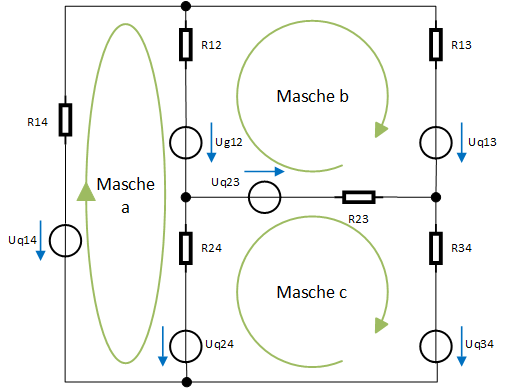
\includegraphics[width=0.7\textwidth]{Bruckenschaltung_mit_Maschen.png}
  \caption{Brückenschaltung mit Maschen}
  \label{fig:brueckenschaltung_maschen}
\end{figure}

Zur Maschenstromanalyse werden zunächst linear unabhängige Maschen aufgestellt. Im nächsten Schritt sind die Spannungssummen zu bilden, die nach dem 2. Kirchhoffschen Gesetz Null ergeben müssen.
  \begin{align}
    &\text{Masche a: }&-U_{q14} &+ U_{q12} &+ U_{q24} &+ (I_a - I_b)R_{12} &+ (I_a - I_c)R_{24} &+ R_{14} I_a &= 0 \nonumber \\
    &\text{Masche b: }&-U_{q12} &+ U_{q13} &- U_{q23} &+ (I_b - I_c)R_{23} &+ (I_b - Ia)R_{12} &+ I_b R_{13}  &= 0 \nonumber \\
    &\text{Masche c: }&-U_{q24} &+ U_{g23} &+ U_{q34} &+ (I_c - I_a)R_{24} &+ (I_c - I_b)R_{23} &+ I_c R_{34} &= 0
    \nonumber \\
  \end{align}
  Aus diesen so erhaltenen Maschengleichungen wird nun ein LGS aufgebaut:
  \begin{equation}
  \begin{tabularx}{14.7cm}{l|c c c | c}
    \textbf{Masche} & $I_a$ & $I_b$ & $I_c$ & \textbf{Quellen} \\ \hline
    \textbf{a: } & $R_{14}+R_{12}+R_{24}$ & $-R_{12}$ & $-R_{24}$ & $U_{q14} - U_{q12} - U_{q24}$ \\
    \textbf{b: } & $-R_{12}$ & $R_{12}+R_{13}+R_{23}$ & $-R_{23}$ & $U_{q12} - U_{q23} + U_{q13}$ \\
    \textbf{c: } & $-R_{24}$ & $-R_{23}$ & $R_{23}+R_{24}+R_{34}$ & $U_{q24} - U_{q23} - U_{q34}$ \\ 
    \multicolumn{5}{c}{$\;$}\\
  \end{tabularx}
  \end{equation}
  
  Dies lässt sich als Matrix einfacher darstellen:
  \begin{align}
    \left(
      \begin{array}{c c c}
      R_{14}+R_{12}+R_{24} & -R_{12} & -R_{24} \\
      -R_{12} & R_{12}+R_{13}+R_{23} & -R_{23} \\
      -R_{24} & -R_{23} & R_{23}+R_{24}+R_{34} \\
      \end{array}
    \right) \cdot \vecT{I_a \\ I_b \\ I_c} \nonumber \\
    = \vecT{U_{q14} - U_{q12} - U_{q24} \\ U_{q12} - U_{q23} + U_{q13} \\U_{q24} - U_{q23} - U_{q34}}
  \end{align}
  
  Diese Matrix lässt sich nun am einfachsten mit der Cramerschen Regel lösen. Da es sich um eine $3\times 3$ Matrix handelt, kann bequem mit der Sarruschen Regel gearbeitet werden.\newline
  Es gilt zunächst die Cramersche Regel:
  \begin{align}
    I_a = \frac{\det D_a}{\det D} \qquad \qquad I_b = \frac{\det D_b}{\det D} \qquad \qquad I_c = \frac{\det D_c}{\det D}
  \end{align}
  Die Determinanten werden über die Sarrussche Regel bestimmt:
  \begin{align}
    \det X &= \left|
      \begin{array}{c c c}
      X_{aa} & X_{ab} & X_{ac}\\
      X_{ba} & X_{bb} & X_{bc}\\
      X_{ca} & X_{cb} & X_{cc}\\
      \end{array}
    \right|    
    = \left|
      \begin{array}{c c c}
      \colGreen{X_{aa}} & \colGreen{X_{ab}} & \colGreen{X}_{\colBlue{ac}}\\
      X_{ba} & \colGreen{X}_{\colBlue{bb}} & \colGreen{X}_{\colBlue{bc}}\\
      \colBlue{X_{ca}} & \colBlue{X_{cb}} & \colGreen{X}_{\colBlue{cc}}\\
      \end{array}
    \right| 
    \begin{array}{c c}
      \colBlue{X_{aa}} & \colBlue{X_{ab}}\\
      \colGreen{X}_{\colBlue{ba}} & X_{bb}\\
      \colGreen{X_{ca}} & \colGreen{X_{cb}}\\
    \end{array} \nonumber \\
    \nonumber \\
    &\Rightarrow \det X =   \colGreen{X_{aa}} \colGreen{X_{bb}} \colGreen{X_{cc}} 
      + \colGreen{X_{ab}}   \colGreen{X_{bc}} \colGreen{X_{ca}}
      + \colGreen{X_{ac}}   \colGreen{X_{ba}} \colGreen{X_{cb}} \nonumber \\
      &\qquad \qquad \qquad- \colBlue{X_{ca}}    \colBlue{X_{bb}}  \colBlue{X_{ac}} 
      - \colBlue{X_{cb}}    \colBlue{X_{bc}}  \colBlue{X_{aa}}
      - \colBlue{X_{cc}}    \colBlue{X_{ba}}  \colBlue{X_{ab}}
  \end{align}
  
  Für die Berechnung der $Determinanten$ $D_a$, $D_b$ und $D_c$ wird nach der Cramerschen Regel jeweils die Spalte in der Matrix mit dem gesuchten Strom durch die Quellenspalte ausgetauscht.
  
  Allgemein gilt also:
  \begin{flalign}
  &X = \left(
    \begin{array}{c c c}
    X_{aa} & X_{ab} & X_{ac}\\
    X_{ba} & X_{bb} & X_{bc}\\
    X_{ca} & X_{cb} & X_{cc}\\
    \end{array}
  \right) \cdot \vecT{I_a \\ I_b \\ I_c} = \vecT{Y_a \\ Y_b \\ Y_c}  \nonumber \\
  \nonumber \\
  &\Rightarrow \det X_a = 
  \left|
    \begin{array}{c c c}
    Y_a & X_{ab} & X_{ac}\\
    Y_b & X_{bb} & X_{bc}\\
    Y_c & X_{cb} & X_{cc}\\
    \end{array}        
  \right|& \nonumber \\ 
  &= \colGreen{Y_a X_{bb} X_{cc}} + \colGreen{X_{ab}X_{bc}Y_c} + \colGreen{X_{ac} Y_b X_{cb}} - \colBlue{X_{ac} X_{bb} Y_c} - \colBlue{Y_a X_{bc} X_{cb}} - \colBlue{X_{ab} Y_b X_{cc}}& \\
  &\Rightarrow \det X_b = 
  \left|
    \begin{array}{c c c}
    X_{aa} & Y_a & X_{ac}\\
    X_{ba} & Y_b & X_{bc}\\
    X_{ca} & Y_c & X_{cc}\\
    \end{array}        
  \right|& \nonumber \\ 
  &= \colGreen{X_{aa} Y_b X_{cc}} + \colGreen{Y_a X_{bc} X_{ca}} + \colGreen{X_{ac} X_{ba} Y_c} - \colBlue{X_{ac} Y_b X_{ca}} - \colBlue{X_{aa} X_{bc} Y_c} - \colBlue{Y_a X_{ba} X_{cc}}& \\ 
  &\Rightarrow \det X_c = 
  \left|
    \begin{array}{c c c}
    X_{aa} & X_{ab} & Y_a\\
    X_{ba} & X_{bb} & Y_b\\
    X_{ca} & X_{cb} & Y_c\\
    \end{array}        
  \right|& \nonumber \\  
  &= \colGreen{X_{aa} X_{bb} Y_c} + \colGreen{X_{ab} Y_b X_{ca}} + \colGreen{Y_a X_{ba} X_{cb}} - \colBlue{Y_a X_{bb} X_{ca}} - \colBlue{X_{aa} Y_b X_{cb}} - \colBlue{X_{ab}X_{ba} Y_c}&\\
  \nonumber  \\
  %
  &\text{Somit ergibt sich für die einzelnen Ströme:}& \nonumber \\
  %
  \nonumber \\
    &I_a = \frac{\det D_a}{\det D} = \frac{
    \left|
    \begin{array}{c c c}
    Y_a & X_{ab} & X_{ac}\\
    Y_b & X_{bb} & X_{bc}\\
    Y_c & X_{cb} & X_{cc}\\
    \end{array}        
  \right|}{
    \left|
    \begin{array}{c c c}
    X_{aa} & X_{ab} & X_{ac}\\
    X_{ba} & X_{bb} & X_{bc}\\
    X_{ca} & X_{cb} & X_{cc}\\
    \end{array}
    \right|
  }& \nonumber \\
  &= \frac{
    Y_a(X_{bb} X_{cc} - X_{bc}X_{cb}) + Y_b(X_{ac} X_{cb} - X_{ab} X_{cc}) 
  + Y_c(X_{ab} X_{bc} - X_{ac} X_{bb})}{
     X_{aa} X_{bb} X_{cc} + X_{ab} X_{bc} X_{ca} + X_{ac} X_{ba} X_{cb} 
  - X_{ca} X_{bb} X_{ac} - X_{cb} X_{bc} X_{aa} - X_{cc}X_{ba} X_{ab}}& \nonumber \\
  \\  
  %      
  &I_b = \frac{\det D_b}{\det D} = \frac{
    \left|
    \begin{array}{c c c}
    X_{aa} & Y_a & X_{ac}\\
    X_{ba} & Y_b & X_{bc}\\
    X_{ca} & Y_c & X_{cc}\\
    \end{array}        
  \right|}{
    \left|
    \begin{array}{c c c}
    X_{aa} & X_{ab} & X_{ac}\\
    X_{ba} & X_{bb} & X_{bc}\\
    X_{ca} & X_{cb} & X_{cc}\\
    \end{array}
    \right|
  }& \nonumber \\
  &= \frac{
    Y_a(X_{bc} X_{ca} - X_{ba}X_{cc}) + Y_b(X_{aa} X_{cc} - X_{ac} X_{ca}) 
  + Y_c(X_{ac} X_{ba} - X_{aa} X_{bc})}{
     X_{aa} X_{bb} X_{cc} + X_{ab} X_{bc} X_{ca} + X_{ac} X_{ba} X_{cb} 
  - X_{ca} X_{bb} X_{ac} - X_{cb} X_{bc} X_{aa} - X_{cc}X_{ba} X_{ab}}& \nonumber \\
  \end{flalign}
  
  \begin{flalign}      
  &I_c = \frac{\det D_c}{\det D} = \frac{
    \left|
    \begin{array}{c c c}
    X_{aa} & X_{ab} & Y_a\\
    X_{ba} & X_{bb} & Y_b\\
    X_{ca} & X_{cb} & Y_c\\
    \end{array}        
  \right|}{
    \left|
    \begin{array}{c c c}
    X_{aa} & X_{ab} & X_{ac}\\
    X_{ba} & X_{bb} & X_{bc}\\
    X_{ca} & X_{cb} & X_{cc}\\
    \end{array}
    \right|
  }& \nonumber \\
  &= \frac{
    Y_a(X_{ba} X_{cb} - X_{bb}X_{ca}) + Y_b(X_{ab} X_{ca} - X_{aa} X_{cb}) 
  + Y_c(X_{aa} X_{bb} - X_{ab} X_{ba})}{
     X_{aa} X_{bb} X_{cc} + X_{ab} X_{bc} X_{ca} + X_{ac} X_{ba} X_{cb} 
  - X_{ca} X_{bb} X_{ac} - X_{cb} X_{bc} X_{aa} - X_{cc}X_{ba} X_{ab}}& \nonumber\\
  \end{flalign}
  Nach Einsetzen der entsprechenden Werte erhält man somit die Lösungen für die einzelnen Maschenströme.
  \subsection{Knotenspannungsanalyse} \label{sec:knotenspann}
  Bei der Knotenspannungsanalyse(Knotenpotenzialverfahren) wird jedem Knoten $i$ ein Potential $\varphi_i$ gegenüber einem Bezugspotential (in der Regel Masse) zugeordnet. Bei der Knotenspannungsanalyse werden entsprechend die Kotenpotentiale berechnet. Aus der Differenz der Potentiale lässt sich so die Spannung zwischen zwei Knoten bestimmen. Dieses Verfahren eignet sich besonders für die Betrachtung von idealen Stromquellen. Sind Spannungsquellen vorhanden, sollten diese durch Einführung eines endlichen Innenwiderstandes $R_i$ dann in ideale Stromquellen umformuliert werden. Bei der endgültigen Lösung muss dann allerdings zwingend $R_i \rightarrow 0$ beachtet werden.
  \begin{itemize}
    \item $I_{qkl}$ ist die Summe aller Stromquellen zwischen den Knoten $k$ und $l$.
    \item Es ergeben sich bei insgesamt $n$ Knoten insgesamt $n-1$ unabhängige Knotengleichungen. 
  \end{itemize}
  Allgemein ergibt sich damit:
 \begin{equation}
  \begin{tabularx}{14.7cm}{l|c c c c | c}
    \textbf{Knoten} & $\varphi_1$ & $\varphi_2$ & $...$ & $\varphi_{n-1}$ &  \textbf{Quellenstrom in Knoten} \\ \hline
    \textbf{1: }    & $G_{ii}$    & $-G_{12}$   & $...$ & $-G_{1,n-1}$    & $I_{q,1}$ \\
    \textbf{2: }    & $-G_{21}$   & $G_{22}$    & $...$ & $...$           & $I_{q,2}$ \\
    $.$             & $...$       & $...$       & $...$ & $...$           & $...$      \\    
    \textbf{n-1: }  & $...$       & $...$       & $...$ & $G_{n-1,n-1}$   & $I_{q,n-1}$ \\ 
    \multicolumn{6}{c}{$\;$}\\
  \end{tabularx}
  \end{equation}
  
  Wobei gilt:
  \begin{itemize}
    \item $G_{ii}$ ist die Summe aller Leitwerte die mit dem Knoten $i$ direkt verbunden sind und positiv ins Schema einzutragen.
    \item $G_{ij}$ ist die Summe aller Leitwerte zwischen den Knoten $i$ und $j$ und negativ ins Schema einzutragen.
    \item $I_{qi}$ ist die Summe aller durch Stromquellen in den Knoten $i$ fließenden Ströme.
    \item Wurde als Bezugsknoten $\varphi_n = 0$ gewählt gilt für die Knotenspannungen: $U_{kn} = \varphi_k - \varphi n = \varphi_k$.
  \end{itemize}
  %Bruckenschaltung_mit_Knotenspannungsanalyse.png
  \begin{figure}[htbp] 
	  \centering
	  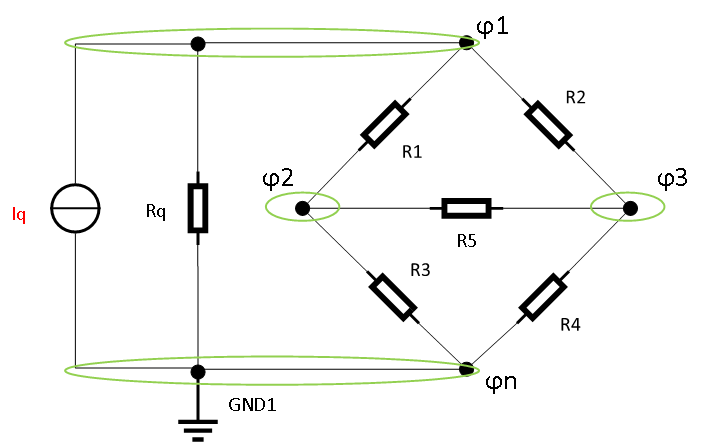
\includegraphics[width=0.7\textwidth]{Bruckenschaltung_mit_Knotenspannungsanalyse.png}
	  \caption{Brückenschaltung mit Knoten}
	  \label{fig:brueckenschaltung_knoten}
  \end{figure}
  
  Diese Schaltung lässt sich einfach mit dem oben beschriebenen Schema als LGS formulieren:
  \begin{equation}
  \begin{tabularx}{14.7cm}{l|c c c c | c}
    \textbf{Knoten} & $\varphi_1$ & $\varphi_2$ & $\varphi_3$ &  \textbf{Quellen} \\ \hline
    \textbf{1: }    & $\frac{1}{R_1} + \frac{1}{R_2} + \frac{1}{R_q}$    & $-\frac{1}{R_1}$    & $-\frac{1}{R_2}$           & $I_q$ \\
    \textbf{2: }    & $-\frac{1}{R_1}$   & $\frac{1}{R_1} + \frac{1}{R_3} + \frac{1}{R_5}$    & $-\frac{1}{R_5}$           & $0$ \\
    \textbf{3: }    & $-\frac{1}{R_2}$    & $-\frac{1}{R_5}$             & $\frac{1}{R_2} + \frac{1}{R_4} + \frac{1}{R_5}$    & $0$ \\ 
    \multicolumn{6}{c}{$\;$}\\
  \end{tabularx}
  \end{equation}
  
  Bzw. als Matrix:
  \begin{align}
    \left(
      \begin{array}{c c c}
      \frac{1}{R_1} + \frac{1}{R_2} + \frac{1}{R_q} & -\frac{1}{R_1}                                & -\frac{1}{R_2} \\
      -\frac{1}{R_1}                                & \frac{1}{R_1} + \frac{1}{R_3} + \frac{1}{R_5} & -\frac{1}{R_5} \\
      -\frac{1}{R_2}                                & -\frac{1}{R_5}                                & \frac{1}{R_2} + \frac{1}{R_4} + \frac{1}{R_5} \\
      \end{array}
    \right) \cdot \vecT{\varphi_1 \\ \varphi_2 \\ \varphi_3} \nonumber \\
    = \vecT{I_q \\ 0 \\0}
  \end{align}
  
  \subsection{Superpositionsprinzip nach Helmholtz}
  Bei Netzwerken mit ausschließlich linearen Netzwerken kann die Berechnung vereinfacht werden, in dem die Spannungsquellen/Stromquellen einzeln betrachtet werden, d.h. es werden immer alle Quellen bis auf eine \dq ausgeschaltet \dq betrachtet. Hierbei gilt für die nichtaktiven Quellen:
  \begin{itemize}
    \item Ideale Spannungsquelle: Kurzschließen
    \item Ideale Stromquelle    : \dq Offen lassen \dq, d.h. Leerlauf  
  \end{itemize}
  Es werden zunächste alle einzelnen Ströme für Quelle $1$: $I_1', I_2', ..., I_n'$, Quelle $2$:$I_1'', I_2'', ..., I_n''$, ... bis Quelle $n$  im Zustand mit deaktivierten Quellen berechnet. Die Gesamtsröme ergeben sich dann aus 
  \begin{equation}
    I_i = I_i' + I_i'' + ... + i_i^{(n)}
  \end{equation}
\newpage

\section{Das statische elektrische Feld}
  Siehe hierzu insbesondere auch \ref{ss:elFeld}.
  \subsection{Elektrischer Fluss}
  \formTab{Elektrische Flussdichte}{\vv{D} = \varepsilon_0 \varepsilon_r \vv{E}}
  Wird manchmal auch als dielektrische Verschiebung bezeichnet.
  \formTab{Elektrischer Fluss}{\Psi = \intd{A}{\;} \vv{D} d\vv{A}}
  \formTab{Elektrischer Fluss durch Kugeloberfläche}{\Psi_K = |\vv{D}|A = Q}
  \subsection{Elektrische Dipole}
  \formTab{Dipolmoment}{\vv{p} = Q \vv{r_{21}} \Rightarrow |\vv{p}| = Qd}
  
  \subsection{Kapazitäten}
  \formTab{Kapazität}{C = \fracd{Q}{U}}
  \formTab{Gespeicherte Energie}{W = \frac{1}{2}C U_0^2}
  \subsubsection{Plattenkondensatoren}
  \formTab{Kapazität ohne Dielektrikum}{C = \fracd{Q}{U} = \varepsilon_0 \fracd{A}{d}}
  \formTab{Kapazität mit Dielektrikum}{C = \fracd{Q}{U} = \fracd{D \cdot A}{E \cdot d} = \fracd{\varepsilon_0 \varepsilon_r A}{d}}
  \formTab{Feld mit Dielektrikun}{E = |\vv{E}| = \fracd{U}{d} = \fracd{D}{\varepsilon_0 \varepsilon_r} = \fracd{Q}{A \varepsilon_0 \varepsilon_r}}
  \formTab{Spannung}{U = E \cdot d = \fracd{Q d}{A \varepsilon_0 \varepsilon_r}}
  \formTab{Flussdichte}{D = \fracd{\varepsilon_0 \varepsilon_r U}{d}}
  \formTab{Verhältnis}{\fracd{Q}{A} = \fracd{\varepsilon_0 \varepsilon_r U}{d} \leftrightarrow \frac{\varepsilon_0 \varepsilon_r A}{d} = C}
  \subsubsection{Kugelkondensator}
  \formTab{Kapazität}{C = \fracd{Q}{U} = 4 \pi \varepsilon_0 \fracd{r_i r_a}{r_i + r_a}}
  \subsubsection{Zylinderkondensator}
  \formTab{Feld}{E = \fracd{Q}{2\pi \varepsilon_0 \varepsilon_r}}
  \formTab{Kapazität}{C = \fracd{Q}{U} = 2 \pi \varepsilon_0 l \fracd{1}{ln\left(\fracd{r_a}{r_i}\right)}}
  \formTab{Kapazitätsbelag}{C' = \frac{C}{l} = \fracd{2 \pi \varepsilon_0}{ln\left(\fracd{r_a}{r_i}\right)}}
  \subsubsection{Kapazitiver Schaltungen}
  \formTab{Spannugsteiler(a)}{\fracd{U_1}{U_2} = \fracd{\frac{Q_1}{C_2}}{\frac{Q_1}{C_1}} = \fracd{C_2}{C_1}}
  \formTab{Spannungsteiler(b)}{\fracd{U_3}{U_1} = \fracd{C_2}{C_2 + C_3}}
  \formTab{Reihenschaltung(a)}{C_g = \fracd{1}{\sum\limits_{k=1}^n \frac{1}{C_k}}}
  \formTab{Ladungserhaltung(b)}{Q_1 = Q_2 = ... = Q_n}
  \formTab{Parallelschaltung(a)}{C_g = \displaystyle\sum\limits_{k=1}^n C_k}
  \formTab{Parallelschaltung(b)}{Q = Q_1 + Q_2 + ... + Q_n}
  
  \subsection{Ladevorgang}
  \formTab{Strom}{i(t) = C \fracd{d u_C (t)}{dt}}
  \formTab{Spannung Widerstand}{u_R (t) = R C \fracd{d u_C (t)}{dt}}
  \formTab{Ladezeitkonstante}{\tau = RC}
  \formTab{Zeitverlauf der Spannung}{u_c (t) = U_0 \left(1-e^{-\fracd{t}{\tau}}\right)}
  \formTab{Zeitverlauf des Stroms}{i(t) = C \fracd{d u_C (t)}{dt} = C \fracd{U_0}{\tau} e^{-\fracd{t}{\tau}} = \fracd{U_0}{R} e^{-\fracd{t}{\tau}} = I_0 e^{-\fracd{t}{\tau}}}
  \formTab{Leistung}{p(t) = U_0 i(t) = \fracd{U_0^2}{R} e^{-\fracd{t}{\tau}}}
  \formTab{Entnommene Energie}{W_Q = U_0^2 C}
  \formTab{Gespeicherte Energie}{W_C = \frac{1}{2} U_0^2 C}
  
  \subsection{Entladevorgang}
  \formTab{Zeitverlauf der Spannung}{u_c (t) = U_0 e^{-\fracd{t}{\tau}}}
  \formTab{Zeitverlauf des Stgroms}{i(t) = C \fracd{d u_C (t)}{dt} =  - \fracd{U_0}{R} e^{-\fracd{t}{\tau}} = -I_0 e^{-\fracd{t}{\tau}}}
  \newpage
\section{Das statische magnetische Feld}
  \subsection{Lorentzkraft und Flussdichte}
  \formTab{Lorentzkraft(a)}{\vv{F_L} = q(\vv{v} \times \vv{B}}
  \formTab{Lorentzkraft(b)}{|\vv{v} \times \vv{B}| = |\vv{v}| |\vv{B}| \sin \alpha}
  \formTab{Magnetische Flussdichte}{\vv{B} = \fracd{\vv{F_L} \times \vv{v}_{max}}{q|\vv{v}_{max}|^2} = \mu_0 \mu_r \vv{H} = \fracd{\phi}{A} = \fracd{wI}{R_m A_i}}
  \subsection{Magnetischer Fluss, Feldstärke und Durchflutung}
  \formTab{Magnetischer Fluss}{\phi = \intd{A}{\;} \vv{B} d\vv{A}}
  \formTab{Magnetische Feldstärke}{\vv{H} = \fracd{\vv{B}}{\mu_0 \mu_r} = \fracd{\phi}{\mu_0 \mu_r A} = \fracd{wI}{R_m A \mu_0 \mu_r}}
  \formTab{Durchflutungsgesetz}{\displaystyle\oint_S \vv{H} \dr = \sum_n I_n = Iw = U_{m,q}}
  Das Durchflutungsgesetz heißt auch das Ampersche Gesetz.
  \subsection{Stromdurchflossene Leiter}
  \formTab{Lorentzkraft(c)}{\vv{F_L} = I (\vv{l} \times \vv{B})}
  \subsubsection{Leiterschleife}
  \formTab{Magnetisches Dipolmoment}{\vv{m} = \mu_0 I \vv{A}}
  \formTab{Drehmoment}{\vv{T} = \fracd{1}{\mu_0} \vv{m} \times \vv{B} = 2 \fracd{w}{2} I l |\vv{B}| \sin \alpha}
  
  \subsection{Magnetische Reluktanz}
  Allgemeine Definition:
  \formTab{Reluktanz(a)}{R_m = \fracd{U_m}{\phi}}
  \formTab{Reluktanz(b)}{R_m = \fracd{l}{\mu_0 \mu_r A}}
  \formTab{Magnetische Spannung}{U_m = \phi R_m}
  \formTab{Magnetischer Fluss}{\phi = \fracd{U_{q,m}}{R_m}}
  
  \subsection{Luftspalt}
   \formTab{Luftspaltgerade}{B_M = -\mu_0 H_M \fracd{l_M A_L}{l_L A_M}}
   \formTab{Flussdichte}{B_L = B_M \fracd{A_M}{A_L}}
   \formTab{Fluss}{\phi_m = B_m A_L}
   \formTab{Optimaler Querschnitt}{A_{M,opt} = \fracd{A_L B_L}{B_{M,opt}}}
   \formTab{Optimale Länge}{l_{M,opt} = \fracd{l_L B_L}{\mu_0 |H_{M,opt}|}}
   \newpage
\section{Zeitlich veränderliche Felder}
  \subsection{Allgemeines Induktionsgesetz}
  \formTab{Induktionsgesetz}{\displaystyle\oint\limits_S \vv{E}\dr = -\displaystyle\oint\limits_A \fracd{d\vv{B}(t)}{dt} d\vv{A} \formTnQQQ  = -\displaystyle\oint\limits_s (\vv{u}(\vv{r})\times \vv{B}(t))\dr - \fracd{d}{dt} \intd{A}{\;} \vv{B}(t)d\vv{A}}
  \formTab{Magnetischer Fluss}{\phi(t) = \intd{A}{\;} \vv{B}(t)d\vv{A}}
  \formTab{Induktion vereinfacht}{U_{ind} = -\fracd{d \phi (t)}{dt}}
  
  \subsection{Induktivität einer Spule}
  \formTab{Spannung}{u(t) = L \fracd{d i(t)}{dt}}
  \formTab{Induktivität}{L = \fracd{\mu_{FE} A_{FE}}{l_{FE}}w^2 = \fracd{\Psi(t)}{i(t)}}
  \formTab{Magnetischer Fluss}{\phi(t) = \fracd{L}{w}i(t)}
  \formTab{Flussverkettung}{\Psi(t) = w \phi (t) = L i(t)}
  
  \subsubsection{Ringspule}
  \formTab{Reluktanz}{R_m = \fracd{2 \pi R - h}{\mu_0 \mu_r A}}
  \formTab{Induktivität}{L = w^2 G_m = \fracd{w^2}{R_m} = w^2 \fracd{\mu_0 \mu_r A}{2 \pi R + h(\mu_r -1)}}
  
  \subsubsection{Hubmagnet}
  \formTab{Fläche Innen}{A_i = \pi (2r_i b + b^2)}
  \formTab{Fläche Aussen}{A_a = \pi)2 r_a b - b^2)}
  
  \subsection{Magnetische Energie}
  \formTab{Momentanleistung}{p(t) = u(t) i(t) = L i(t) \fracd{d i(t)}{dt}}
  \formTab{Energie}{W = \fracd{1}{2}L i_0^2 = \fracd{1}{2} \Psi i_0}  
  
  \subsection{Schaltungen von Induktivitäten}
  \formTab{Reihenschaltung}{L_g = \displaystyle\sum\limits_(n = 1)^k L_n}
  \formTab{Parallelschaltung}{L_g = \fracd{1}{\sum\limits_{n = 1}^{k} \frac{1}{L_n}}}
  \formTab{Reihenschaltung gekoppelt}{L_g = L_1 + L_2 \pm L_{12}}
  \formTab{Parallelschaltung gekoppelt}{L_g = \fracd{L_1 L_2 - L_{12}^2}{L_1 + L_2 \mp 2 L_{12}^2}}
  \formTab{Stromteiler}{\fracd{\phi_1}{\phi_g} = \fracd{R_{m,g}}{R_{m,1}}}
  
  \subsection{Einschaltvorgang}
  \formTab{Ladezeitkonstante}{\tau = \fracd{L}{R}}
  \formTab{Spannung}{u_L (t) = L \fracd{d i(t)}{dt} = U_0 e^{-\fracd{t}{\tau}}}
  \formTab{Strom}{i(t) = \fracd{U_0}{R} \left( 1 - e^{-\fracd{t}{\tau}}\right)}
  
  \subsection{Abschaltvorgang}
  \formTab{Spannung}{u_L (t) = L \fracd{d i(t)}{dt} =  - I_0 R e^{-\fracd{t}{\tau}}}
  \formTab{Strom}{i(t) = I_o e^{-\fracd{t}{\tau}}}
  \newpage
\section{Anhänge}
	\subsection{Abkürzungen/Formelzeichen} \label{ch:names}
	\renewcommand{\arraystretch}{1.5}
	\begin{longtable} {|p{2cm}|p{3cm}|p{8.4cm}|} \hline
	% Definition des Tabellenkopfes auf der ersten Seite
	%Spaltenbezeichnungen
	\textbf{Zeichen} & \textbf{Einheit} & \textbf{Bedeutung} \\
	\hline
	\endfirsthead % Erster Kopf zu Ende
	% Definition des Tabellenkopfes auf den folgenden Seiten
	\caption{Abkürzungen/Formelzeichen}\\ \hline
	%Spaltenbezeichnungen
	\textbf{Zeichen} & \textbf{Einheit} & \textbf{Bedeutung} \\
	\hline
	\endhead % Zweiter Kopf ist zu Ende
	\multicolumn{3}{r}{Fortsetzung auf Folgeseite}\\
	\endfoot
	\hline
	%\multicolumn{3}{r}{Ende} \\
	\endlastfoot
	
	%a-g
	$A$ & $m^2$ & Fläche \\ \hline
	$a$ & $\frac{m}{s^2}$ & Beschleunigung \\ \hline
	$b$ & $\frac{cm^2}{Vs}$ & Ladungsträgerbeweglichkeit \\ \hline
	$d$ & $m$ & Dicke \\ \hline
	$D_n$ & $\frac{m^2}{s}$ & Diffusionskonstante für Elektronen \\ \hline
	$D_p$ & $\frac{m^2}{s}$ & Diffusionskonstante für Löcher \\ \hline
	$e$ & $C$ & Elementarladung \\ \hline
	$E$ & $\frac{N}{C} = \frac{VAs}{mAs} = \frac{V}{m}$ & Elektrische Feldstärke \\ \hline
	$E_c$ & $eV$ & Leitungsbandkante \\ \hline
	$E_F$ & $eV$ & Fermi-Energie \\ \hline
	$E_g$ & $eV$ & Energie der Bandlücke \\ \hline
	$E_v$ & $eV$ & Valenzbandkante \\ \hline
	$f$ & $Hz$ & Frequenz \\ \hline
	$\vec{F}$ & $N = \frac{kgm}{s^2}$ & Kraft \\ \hline
	$G$ & $\frac{A}{V} = \frac{1}{\Omega} = S$ & Leitwert \\ \hline
	
	%h-n
	$h$ & $eVs$ & Plank-Konstante\\ \hline
	$\hbar$ & $eVs$ & Planksches Wirkungsquantum \\ \hline
	$i$ & $A$ & Elektrischer Strom \\ \hline
	$j$ & $\frac{A}{m2}$ & Elektrische Stromdichte \\ \hline
	$J_n$ & $\frac{A}{m2}$ & Elektronenstromdichte \\ \hline
	$J_p$ & $\frac{A}{m2}$ & Löcherstromdichte \\ \hline
	$J_{diff}$ & $\frac{A}{m2}$ & Diffusionsstromdichte \\ \hline
	$J_{part}$ & $\frac{A}{m2}$ & Partikelstromdichte \\ \hline
	$J_to$ & $\frac{A}{m2}$ & Totale Stromdichte \\ \hline
	$J_r$ & $\frac{A}{m2}$ & Rekombinationsstromdichte \\ \hline
	$J_{drift}$ & $\frac{A}{m2}$ & Driftstromdichte \\ \hline
	$l$ & $m$ & Länge \\ \hline
	$L$ & $m$ & Minoritätsladungsträgerdiffusionslänge \\ \hline
	$L_n$ & $m$ & Diffusionslänge Elektronen \\ \hline
	$L_p$ & $m$ & Diffusionslänge Löcher \\ \hline
	
	%m-u
	$n$ & ... & Elektronenkonzentration \\ \hline
	$n_i$ & ... & Intrinsische Ladungsträgerdichte \\ \hline
	$n_{id}$ & ... & Idealität einer Diode \\ \hline
  $N_A$ & $m^{-3}$ & Akzeptorendichte \\ \hline
  $N_D$ & $m^{-3}$ & Donatorendichte \\ \hline
	$N_C$ & $cm^{-3}$ & Effektive Zustandsdichte der Elektronen \\ \hline
	$N_V$ & $cm^{-3}$ & Effektive Zustandsdichte der Löcher \\ \hline
	$p$ & ... & Lochkonzentration \\ \hline
	$q$ & $C$ & Probeladung (in der Regel = $e$) \\ \hline
	$\vec{r}$ & $m$ & Weg \\ \hline
	$r$ & $\Omega$ & Differentieller Widerstand \\ \hline
	$R$ & $\Omega$ & Widerstand \\ \hline
	$R_F$ & $\frac{\Omega}{square}$ & Flächenwiderstand \\ \hline 
	$U$ & $V$ & Elektrische Spannung \\ \hline
	$U_g$ & $V$ & Gesamtspannung \\ \hline
	 
	%v-z
	$v$ & $\frac{m}{s}$ & Geschwindigkeit \\ \hline
	$v_D, v_d$ & $\frac{m}{s}$ & Driftgeschwindigkeit \\ \hline
	$w$ & $m$ & Weite bzw. Breite  \\ \hline
	$W$ & $Ws = J = \frac{kgm^2}{s^2}$ & Arbeit bzw. Energie \\ \hline
	
	%griechisch
	$\alpha$ & $\frac{1}{^{\circ} C}$ & Temperturkoeffizient des Ohmwiderstandes \\ \hline
	$\nu$ & $Hz$ & Hier Frequenz der Welle \\ \hline
	$\rho$ & $\frac{V cm}{A} = \Omega  cm$ & Spezifischer Widerstand \\ \hline
	$\rho_e$ & ... & Ladungsdichte \\ \hline
	$\kappa$ & $\frac{1}{\Omega cm} = \frac{S}{cm}$ & Spezifische Leitfähigkeit \\ \hline
	$\varepsilon_0$ & $\frac{As}{Vm}$ & Dielektrizitätskonstante im Vakuum \\ \hline
	$\varphi$ & $V$ & Elektrisches Potential \\ \hline
	$\tau$ & $s$ & Stoßzeit \\ \hline
	$\tau$ & $s$ & Minoritätsladungsträgerlebensdauer \\ \hline
	$\mu$ & $\frac{cm^2}{Vs}$ & Beweglichkeit \\ \hline
	%Sonderzeichen
	\end{longtable}
	\renewcommand{\arraystretch}{1}
	
	\subsection{Konstanten} \label{ch:constants}
	\renewcommand{\arraystretch}{1.5}
	
	\begin{longtable} {|p{0.6cm}|p{4.4cm}|p{8.4cm}|} \hline
	% Definition des Tabellenkopfes auf der ersten Seite
	%Spaltenbezeichnungen
	\textbf{Ze.} & \textbf{Wert} & \textbf{Bedeutung}\\
	\hline
	\endfirsthead % Erster Kopf zu Ende
	% Definition des Tabellenkopfes auf den folgenden Seiten
	\caption{Konstanten}\\ \hline
	%Spaltenbezeichnungen
	\textbf{Ze.} & \textbf{Wert} & \textbf{bedeutung}\\
	\hline
	\endhead % Zweiter Kopf ist zu Ende
	\multicolumn{3}{r}{Fortsetzung auf Folgeseite}\\
	\endfoot
	\hline
	%\multicolumn{3}{r}{Ende} \\
	\endlastfoot
	
	%a-g
	$c$ & $2,998...\cdot 10^8 \bracks{frac{m}{s}}$ & Lichtgeschwindigkeit\\ \hline
	$e,q$ & $1,602176...\cdot 10^{-19}\bracks{C}$ & Elementarladung\\ \hline
	%h-n
	$h$ & $6,63 \cdot 10^{-34} \bracks{Js}$ & Planck-Konstante\\ \hline
	$h$ & $4,136...\cdot 10^{-15} \bracks{eVs}$ & Planck-Konstante\\ \hline
	$\hbar$ & $\frac{h}{2\pi}$ & Plancksches Wirkungsquantum\\ \hline
	$k$ & $8,6173 \cdot 10^{-5} \bracks{\frac{eV}{K}}$ & Boltzmann Konstante\\ \hline
	$kT$ & $25,85 \bracks{meV}$ & mit der Boltzmann Konstante und $T=300K$ \\ \hline
	%m-u
	$m_0$ & $9,11 \cdot 10^{-31} \bracks{kg}$ & Elektronenmasse\\ \hline
	$m^*_{si}$ & $0,2 \cdot m_0$ & Effektive Masse Silizium \\ \hline
	$m^*_{ge}$ & $0,1 \cdot m_0$ & Effektive Masse Germanium \\ \hline
	$N_V$ & $1,04\cdot 10^{19}cm^{-3}$ & Zustandsdichte im VB Silizium \\ \hline
	$N_C$ & $2,80\cdot 10^{19}cm^{-3}$ & Zustandsdichte im LB Silizium \\ \hline
	$R$ & $1,09737 \cdot 10^7 m^{-1} $ & Rydbergkonstante\\ \hline
	%v-z
	
	%griechisch
	$\varepsilon_0$ & $8,854..\cdot 10^{-12}\bracks{\frac{As}{Vm}}$ & Dielektrizitätskonstante des Vakuuums \\ \hline
	$\varepsilon_{Si}$ & $11,90$ & Korrekturfaktor Dielektrizitätskonstante für Silizium\\ \hline
	$\varepsilon_{Ge}$ & $16$ & Korrekturfaktor Dielektrizitätskonstante für Germanium\\ \hline
	$\varepsilon_{Si0_2}$ & $3,9$ & Korrekturfaktor Dielektrizitätskonstante für Si02\\ \hline
	%Sonderzeichen
	\end{longtable}
	\renewcommand{\arraystretch}{1}
	
	\subsubsection{Spezifische Widerstände $\left[\mu \Omega cm \right]$}
\begin{tabularx}{14.7cm}{|X|X|X|X|X|X|}\hline
Cu & Au & Ag & Al & Cr & Ta \\ \hline
$1,673$ & $2,35$ & $1,59$ & $2,655$ & $14,1$ & $13,5$ \\ \hline
\end{tabularx}

\subsubsection{Temperaturkoeffizienten $\alpha$ ohmscher Widerstände bei $20^{\circ} C$ in $\left[\frac{1}{^{\circ} C} \right]$}
\begin{tabularx}{14.7cm}{|X|X|X|X|X|X|X|} \hline
Cu & Ag & Au & Al & Ta & Ni & Konst. \\ \hline
$3,9 * 10^{-3}$ & $3,8 * 10^{-3}$ & $3,7 * 10^{-3}$ & $4,0 * 10^{-3}$ & $3,3 * 10^{-3}$ & $6,0 * 10^{-3}$ & $1,0 * 10^{-3}$ \\ \hline
\end{tabularx}
\subsection{SI-Basiseinheiten}
\begin{tabular} {|c|c|c|}\hline
Bezeichnung & Einheit & Bedeutung \\ \hline
Meter & m & Einnheit der Länge \\ \hline
Kilogramm & kg & Einheit der Masse \\ \hline
Sekunde & s & Einheit der Zeit \\ \hline
Ampere & A & Eineit der Stromstärke \\ \hline
Kelvin & K & Einheit der Temperatur \\ \hline
Mol & mol & Einheit der Stoffmenge \\ \hline
Candela & cd & Einheit der Lichtstärke \\ \hline
\end{tabular}

\subsection{Vorsatzzeichen}
\begin{tabular} {|c|c|c|c|c|c|} \hline
Name & Zeichen & Zehnerpotenz & Name & Zeichen & Zehnerpotenz \\ \hline
Yotta & Y & $10^{24}$ & Dezi & d & $10^{-1}$ \\ \hline
Zetta & Z & $10^{21}$ & Centi & c & $10^{-2}$ \\ \hline
Exa & E & $10^{18}$ & Milli & m & $10^{-3}$ \\ \hline
Peta & P & $10^{15}$ & Mikro & $\mu$ & $10^{-6}$ \\ \hline
Tera & T & $10^{12}$ & Nano & n & $10^{-9}$ \\ \hline
Giga & G & $10^{9}$ & Piko & p & $10^{-12}$ \\ \hline
Mega & M & $10^{6}$ & Femto & f & $10^{-15}$ \\ \hline
Kilo & k & $10^{3}$ & Atto & a & $10^{-18}$ \\ \hline
Hekto & h & $10^{2}$ & Zepto & z & $10^{-21}$ \\ \hline
Deka & da & $10^{1}$ & Yokto & y & $10^{-24}$ \\ \hline
\end{tabular}
  
  \newpage
\subsection{Kurzzusammenfassung}
\subsubsection{Elektrostatik}
\begin{figure}[H] 
	  \centering
	  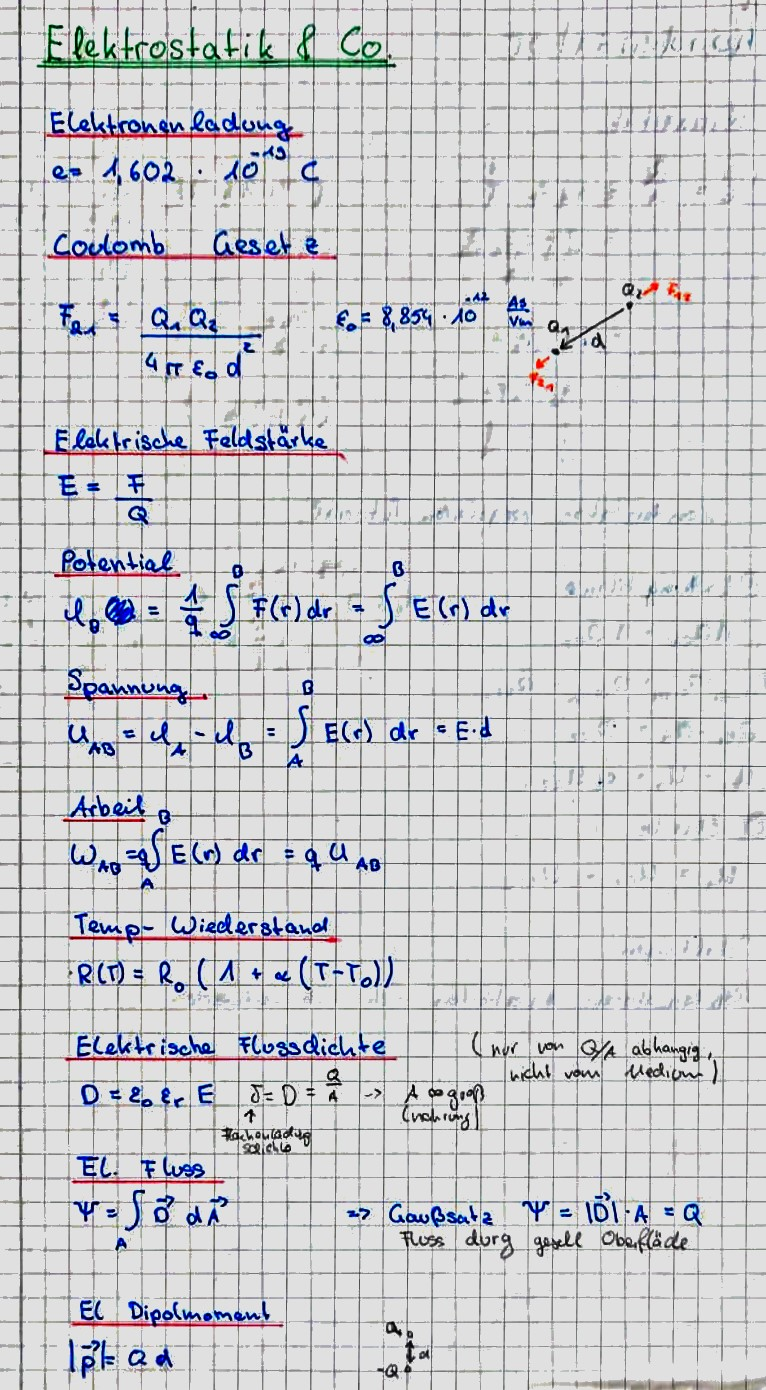
\includegraphics[width=0.75\textwidth]{1_Elektrostatik.jpg}
	  \caption{Kurzzusammenfassung Elektrostatik}
	  \label{fig:elektrostatik}
  \end{figure}
  \newpage
\subsubsection{Kondensator}
\begin{figure}[H] 
	  \centering
	  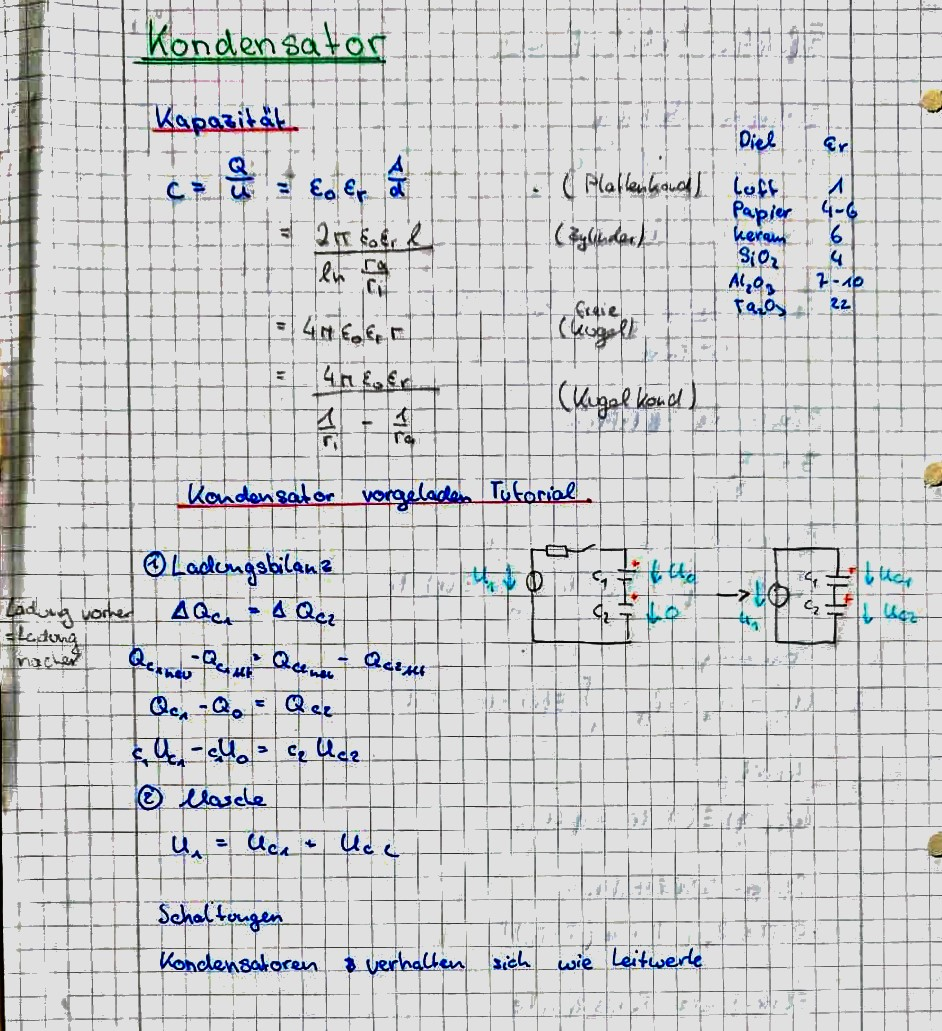
\includegraphics[width=1\textwidth]{2_Kondensator.jpg}
	  \caption{Kurzzusammenfassung Kondensator}
	  \label{fig:Kondensator}
  \end{figure}
  \newpage
  \subsubsection{Magnet 1}
\begin{figure}[H] 
	  \centering
	  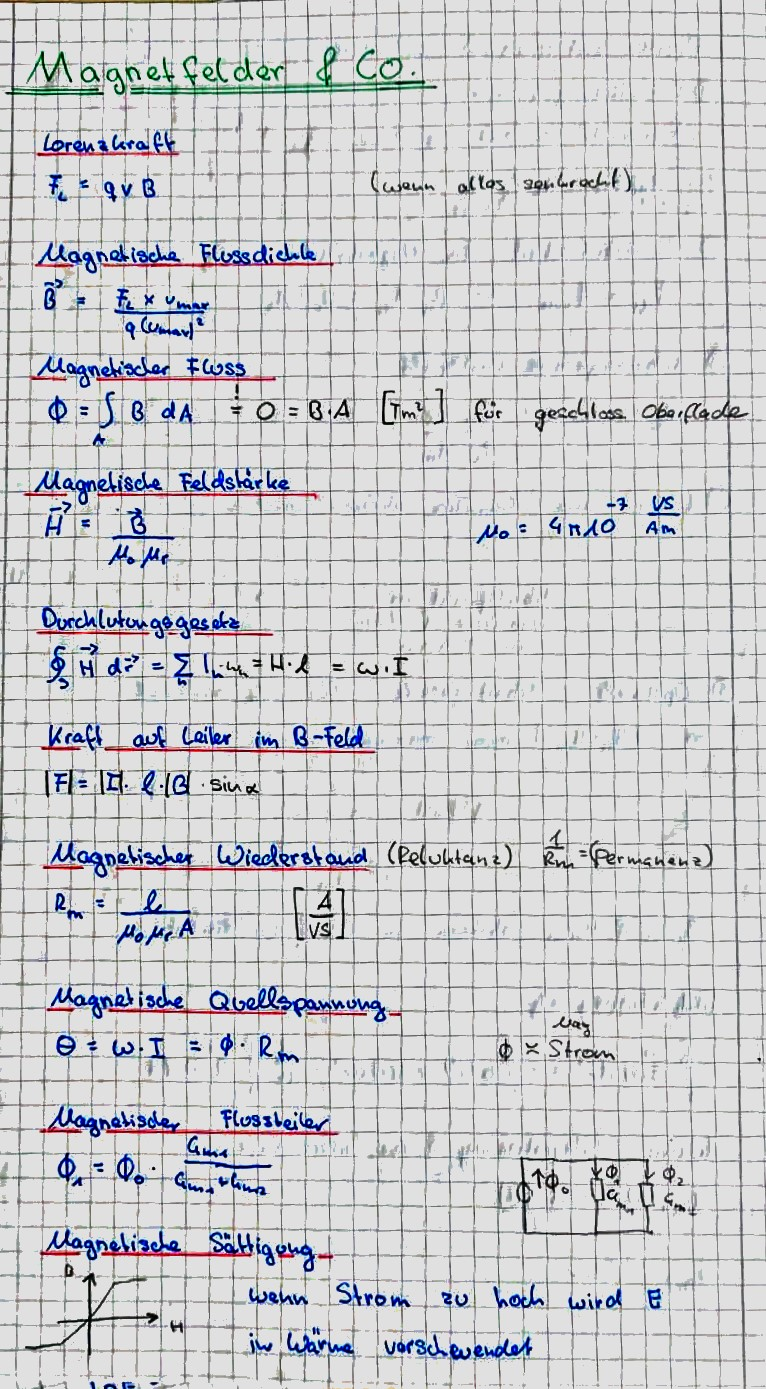
\includegraphics[width=0.8\textwidth]{3_Magnet_1.jpg}
	  \caption{Kurzzusammenfassung Magnet 1}
	  \label{fig:magnet_1}
  \end{figure}
  \newpage
  \subsubsection{Magnet 2}
\begin{figure}[H] 
	  \centering
	  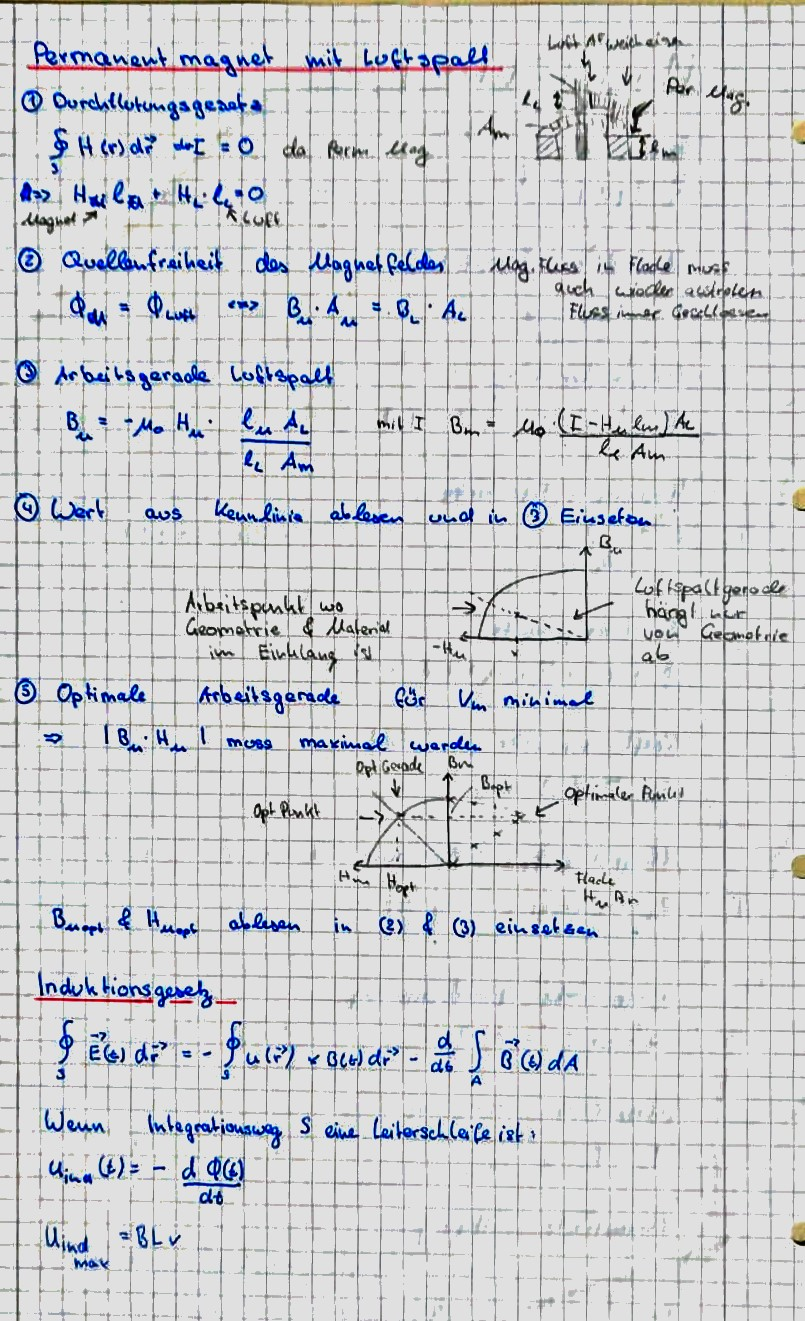
\includegraphics[width=0.87\textwidth]{4_Magnet_2.jpg}
	  \caption{Kurzzusammenfassung Magnet 2}
	  \label{fig:magnet_2}
  \end{figure}
  \newpage
  \subsubsection{Spule}
\begin{figure}[H] 
	  \centering
	  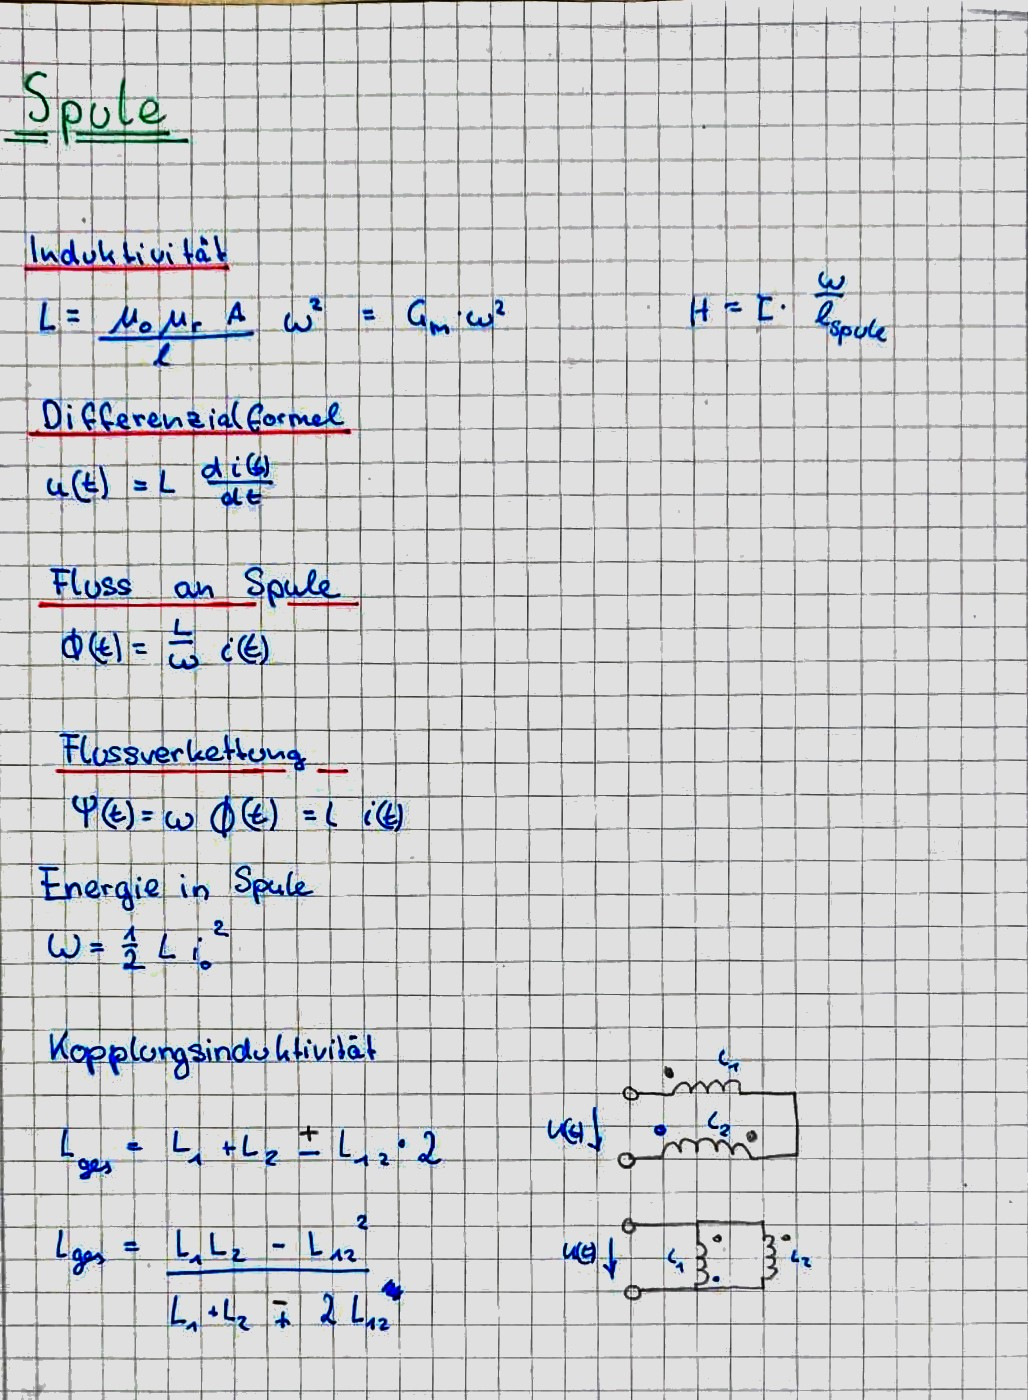
\includegraphics[width=1\textwidth]{5_Spule.jpg}
	  \caption{Kurzzusammenfassung Spule}
	  \label{fig:Spule}
  \end{figure}
  \newpage
  \subsubsection{Komplexe Rechnung}
\begin{figure}[H] 
	  \centering
	  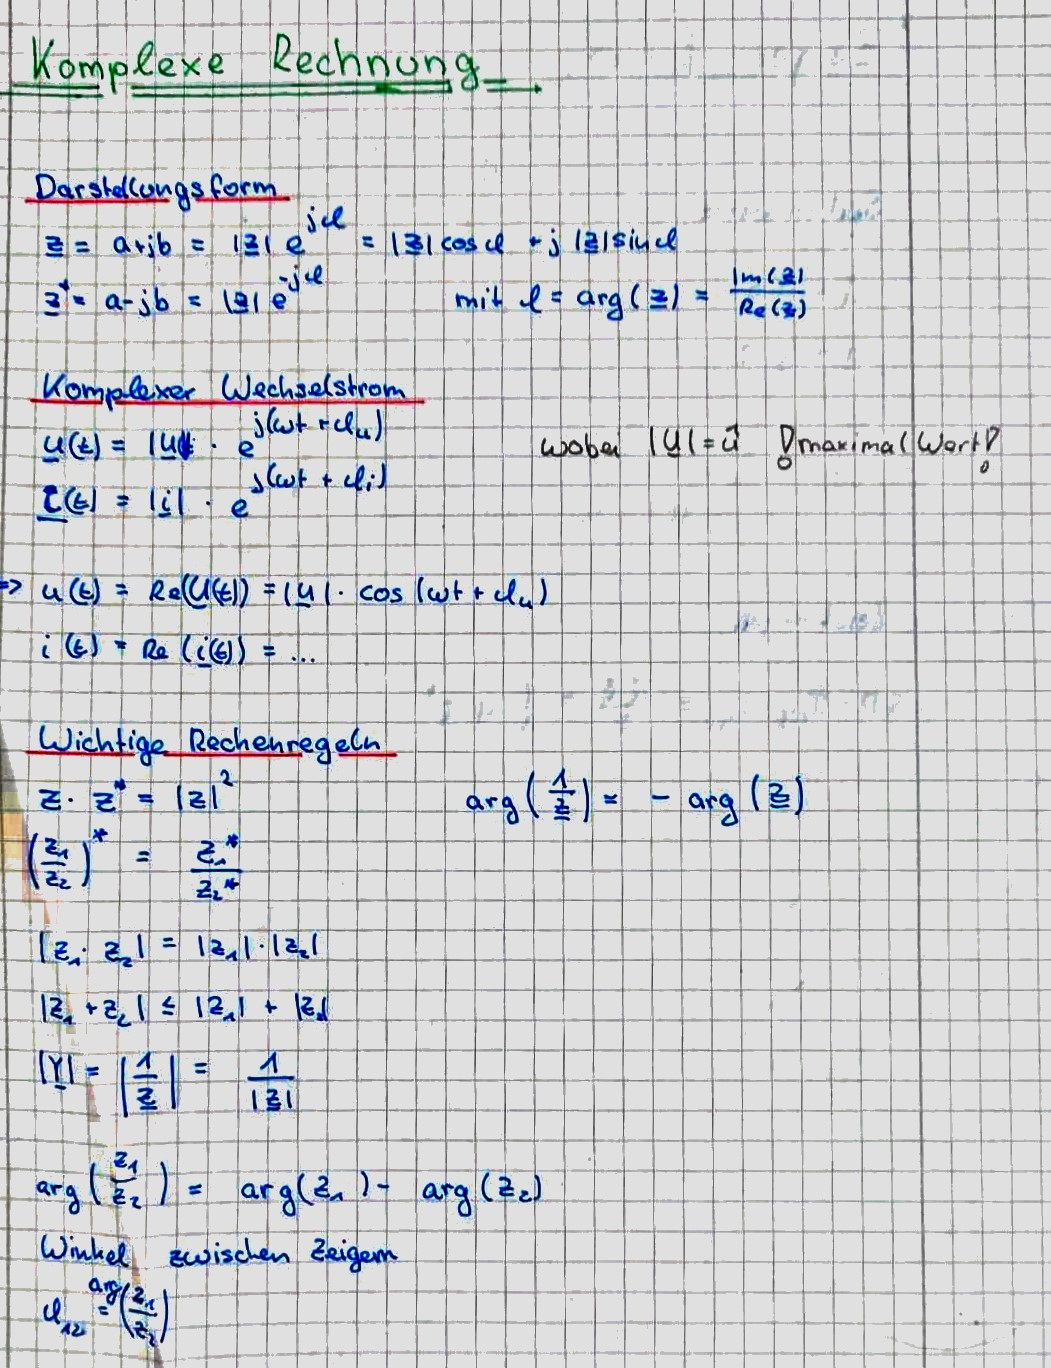
\includegraphics[width=1\textwidth]{6_KomplRechnung.jpg}
	  \caption{Kurzzusammenfassung Komplexe Rechnung}
	  \label{fig:Komplexe Rechnung}
  \end{figure}
  \newpage
  \subsubsection{Zeiger}
\begin{figure}[H] 
	  \centering
	  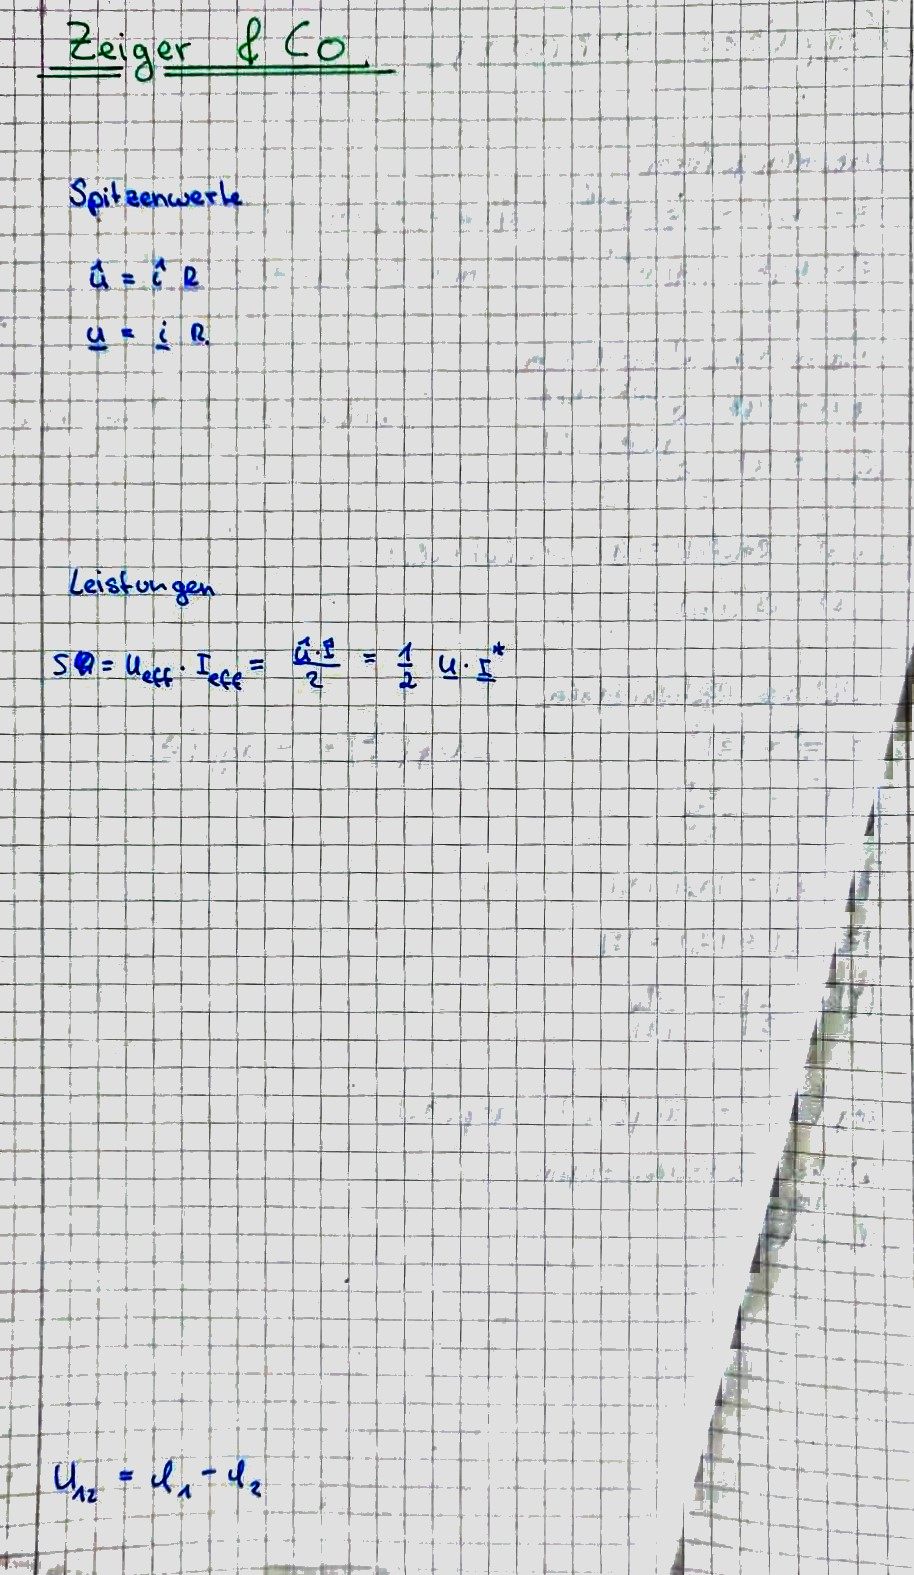
\includegraphics[width=0.85\textwidth]{7_Zeiger.jpg}
	  \caption{Kurzzusammenfassung Zeiger}
	  \label{fig:Zeiger}
  \end{figure}
  \newpage
  \subsubsection{Übertrager}
\begin{figure}[H] 
	  \centering
	  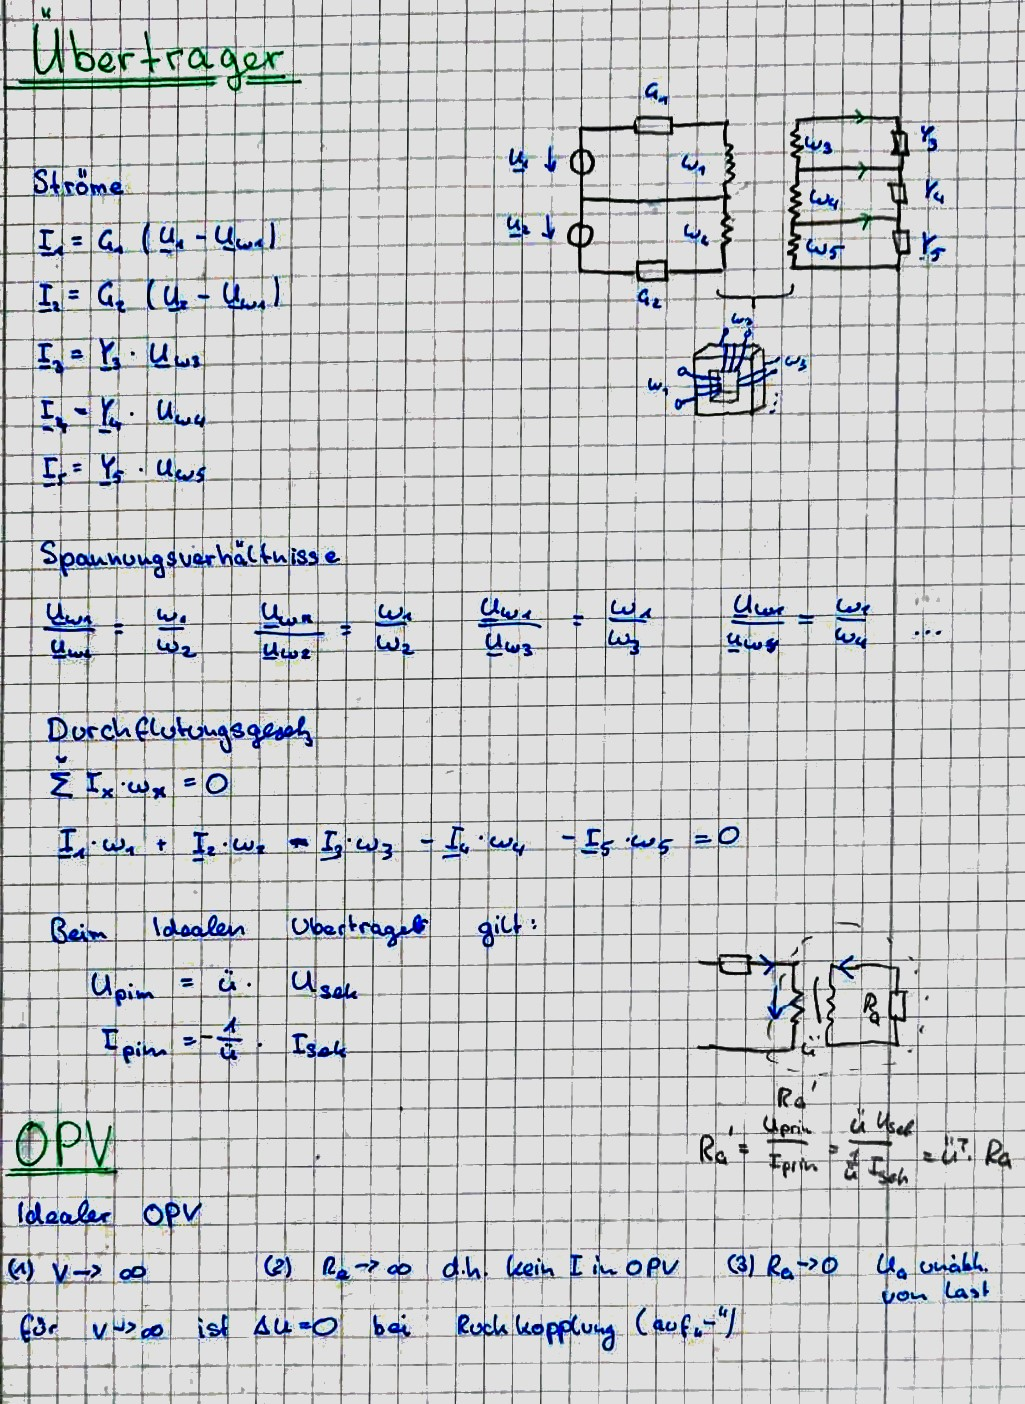
\includegraphics[width=1\textwidth]{8_Uebertrager.jpg}
	  \caption{Kurzzusammenfassung Übertrager}
	  \label{fig:Übertrager}
  \end{figure}
  \newpage
  \subsection{Nachwort}
  Diese Formelsammlung wurde nahezu ausschließlich auf Basis des Grundlagen der Elektrotechnik I-II Scripts von Prof. Dr.-Ing. Norbert Frühauf erstellt. Nahezu sämtliche Formeln und Werte sind direkt dem Script und der Vorlesung entnommen und wurden nicht für diese Sammlung eigenständig hergeleitet. Für ausführlichere Beschreibungen empfehle ich sehr das eben angesprochene Script zu studieren. Diese Formelsammlung ist einzig ein Hilfsmittel für mich und meine Kommilitonen und sehr wahrscheinlich nicht fehlerfrei. Sollten Fehler gefunden werden, würde ich mich sehr freuen wenn man mir das kurz in einer E-Mail (f.leuze@outlook.de) mitteilen würde, damit ich entsprechende Korrekturen vornehmen kann. Die angefügte Kurzformelsammlung wurde freundlicherweise von unserem Elektrotechnik Tutor zur Verfügung gestellt.
  
%\bibliography{lit}

\end{document}